% Ensure that you compile using XeLaTeX !!! PDFTex has problems with some of the packages used
\documentclass[12pt]{article}
\setlength\parindent{0pt}

\usepackage{parskip}
\usepackage[margin=0.5in]{geometry}
\usepackage{fullpage}
\usepackage{moresize}
\usepackage{graphicx}
\usepackage{caption}
\usepackage{subcaption}
\usepackage{float}
\usepackage{xcolor}
\usepackage{soul}
\usepackage{fontspec}
\setmainfont{Doulos SIL}

\begin{document}

\begin{center}
\textbf{{\color{violet}{\HUGE 20201014 Wednesday\\}}}

\textbf{{\color{violet}{\HUGE ALL EXAMS\\}}}

\end{center}
\newpage

\begin{center}
\textbf{{\color{blue}{\HUGE START OF EXAM\\}}}

\textbf{{\color{blue}{\HUGE Student ID: 44715\\}}}

\textbf{{\color{blue}{\HUGE 4:00\\}}}

\end{center}
\newpage

{\large Question 1}\\

Source: Week 3 Handout, Question 3\\

Explain why the additional vowel below either does or does not belong in the phonetic natural class defined by the original set of SNAE vowels.\\

Original set: {[u]}, {[ʊ]}, {[oʊ]}, {[ɔ]}

Addition: {[ɔɪ]}


\newpage

{\large Question 2}\\

Source: Week 4 Discussion\\

Explain why the given feature's value varies across this set of sounds.\\

{[sonorant]}

alveolars


\newpage

\begin{center}
\textbf{{\color{red}{\HUGE END OF EXAM}}}\\

\end{center}
\newpage

\begin{center}
\textbf{{\color{blue}{\HUGE START OF EXAM\\}}}

\textbf{{\color{blue}{\HUGE Student ID: 34548\\}}}

\textbf{{\color{blue}{\HUGE 4:10\\}}}

\end{center}
\newpage

{\large Question 1}\\

Source: Week 3 Handout, Question 3\\

Explain why the additional vowel below either does or does not belong in the phonetic natural class defined by the original set of SNAE vowels.\\

Original set: {[æ]}, {[ɑ]}

Addition: {[ɑʊ]}


\newpage

{\large Question 2}\\

Source: Week 4 Discussion\\

Explain what the given feature’s value is for this class of sounds, and why.\\

{[continuant]}

glottals


\newpage

\begin{center}
\textbf{{\color{red}{\HUGE END OF EXAM}}}\\

\end{center}
\newpage

\begin{center}
\textbf{{\color{blue}{\HUGE START OF EXAM\\}}}

\textbf{{\color{blue}{\HUGE Student ID: 78380\\}}}

\textbf{{\color{blue}{\HUGE 4:20\\}}}

\end{center}
\newpage

{\large Question 1}\\

Source: Week 3 Discussion\\

Describe what the tongue would do / where it would move during each of the vowels in this word.\\

<July>


\newpage

{\large Question 2}\\

Source: Week 2 Handout, Part II\\

Is this a reasonable transcription of this word? Explain why.\\

<mouse>: {[mɔɪs]}


\newpage

\begin{center}
\textbf{{\color{red}{\HUGE END OF EXAM}}}\\

\end{center}
\newpage

\begin{center}
\textbf{{\color{blue}{\HUGE START OF EXAM\\}}}

\textbf{{\color{blue}{\HUGE Student ID: 68382\\}}}

\textbf{{\color{blue}{\HUGE 4:30\\}}}

\end{center}
\newpage

{\large Question 1}\\

Source: Week 2 Handout, Part II\\

Is this a reasonable transcription of this word? Explain why.\\

<loud>: {[lɑud]}


\newpage

{\large Question 2}\\

Source: Homework 1, Question 3(b)\\

Explain why this is or is not a complete phonetic natural class in standard North American English.\\

{[ɔ]}, {[ʊ]}, {[u]}, {[oʊ]}


\newpage

\begin{center}
\textbf{{\color{red}{\HUGE END OF EXAM}}}\\

\end{center}
\newpage

\begin{center}
\textbf{{\color{blue}{\HUGE START OF EXAM\\}}}

\textbf{{\color{blue}{\HUGE Student ID: 74654\\}}}

\textbf{{\color{blue}{\HUGE 4:40\\}}}

\end{center}
\newpage

{\large Question 1}\\

Source: Week 3 Handout, Question 3\\

Explain why the additional vowel below either does or does not belong in the phonetic natural class defined by the original set of SNAE vowels.\\

Original set: {[æ]}, {[ɑ]}

Addition: {[ɑɪ]}


\newpage

{\large Question 2}\\

Source: Week 4 Handout, Part II, Question 3\\

Explain how you would figure out what the Luiseño form is for the morpheme whose meaning is given below. (To be clear: you do NOT need to give me the form itself -- just explain the process of figuring it out.)\\

‘drink’

\begin{figure}[H]
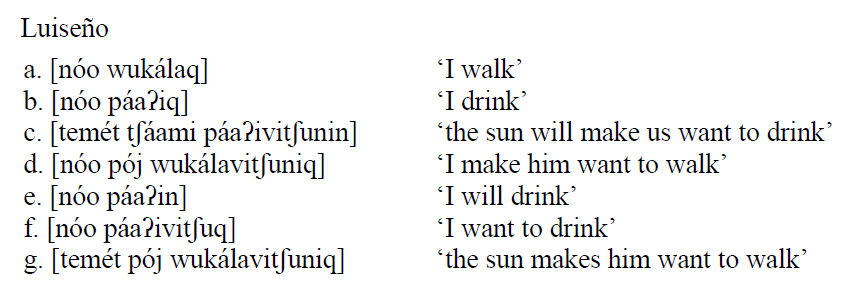
\includegraphics{../images/luiseno.png}
\end{figure}

\newpage

\begin{center}
\textbf{{\color{red}{\HUGE END OF EXAM}}}\\

\end{center}
\newpage

\begin{center}
\textbf{{\color{blue}{\HUGE START OF EXAM\\}}}

\textbf{{\color{blue}{\HUGE Student ID: 99594\\}}}

\textbf{{\color{blue}{\HUGE 4:50\\}}}

\end{center}
\newpage

{\large Question 1}\\

Source: Week 5 Handout, Question 1\\

Explain why we think that languages are not random in terms of their phonology.\\


\newpage

{\large Question 2}\\

Source: Week 3 Handout, Question 3\\

Explain why the additional vowel below either does or does not belong in the phonetic natural class defined by the original set of SNAE vowels.\\

Original set: {[u]}, {[ʊ]}, {[oʊ]}, {[ɔ]}

Addition: {[ɑʊ]}


\newpage

\begin{center}
\textbf{{\color{red}{\HUGE END OF EXAM}}}\\

\end{center}
\newpage

\end{document}

